\documentclass[a4paper,fontset=fandol]{ctexart}

\usepackage{amsmath,amssymb,amsthm,physics,fancyhdr,geometry,hyperref,graphicx,enumitem,upgreek,booktabs}

\geometry{vmargin=2cm,hmargin=2.5cm}

\pagestyle{fancy}
\fancyhf{}
\fancyfoot[C]{\thepage}
\renewcommand{\headrulewidth}{0pt}

\usepackage{titlesec}
\titleformat{\section}
{\normalfont\Large\bfseries}{理论\thesection:}{0.5em}{}

\newcommand{\points}[1]{\par % 确保换行
	\noindent % 取消缩进
	\hfill (#1分)% 右对齐并添加分数
	\vspace{1em}
	}

%\parskip=0.5em

\hypersetup{colorlinks=true,bookmarks=true,bookmarksopen=false,pdfstartview=FitH}

\begin{document}
	{
	\Large\bfseries\noindent 理论:\hspace{0.5em}指导说明
	}
	
	\begin{itemize}
		\item {\bfseries 不要触碰信封, 直到考试开始. }
		
		\item 理论考试时长为5小时, 总分为250分. 
		
		\item 有\textbf{答题纸}用于详细答题, 以及\textbf{草稿纸}用于粗略计算, 这些纸张已经标记了你的学生代码和题目编号. 
		
		\item {\bfseries\itshape 只使用特定题目的答题纸进行答题. 请只在纸张的打印面上书写, 不要使用背面. }如果你在任何纸张上写了不想被评分的内容, 请将其划掉. 
		
		\item 使用尽可能多的数学表达式来帮助评分者更好地理解你的解决方案. 评分者可能不懂你的语言. 如果需要用文字解释某些内容, 请使用简短的短语(如果可能的话, 请使用英语). 
		
		\item 未经允许, 不得离开工作台. 如果你需要任何帮助(计算器故障、需要去洗手间等), 请向监考员示意. 
		
		\item 考试的开始和结束将由监考员指示. 剩余时间将在时钟上显示. 
		
		\item 考试结束时, 你必须立即停止书写. 把所有东西放回信封, 并将其留在桌子上. 
		
		\item 一旦收集完所有信封, 你的向导将引导你离开考场. 
		
		\item 信封内附有常数列表和有用的关系式. 
	\end{itemize}
	
	\newpage
	\section{海王星}
	
	假设海王星将在2024年9月21日处于冲的位置, 计算海王星上一次在北半球春分附近处于冲的位置是哪一年. 假设地球和海王星的轨道是圆形的. 
	
	\points{5}
	
	\section{磁场}
	
	在一颗白矮星的光谱中观察到了波长为 $\lambda = 600\text{ nm}$ 的发射线. 假设它起源于自由非相对论电子与磁场的相互作用, 
	\begin{enumerate}[label=(\alph*)]
		\item 计算该场的磁通密度;
		
		\item 估计另一条谱线的波长, 其发现可以证实这些线起源于与磁场相互作用的等离子体粒子. 
	\end{enumerate}
	
	\points{5}
	
	\section{微引力透镜效应}
	
	一颗位于银河系中心的微弱亚矮星($I=20.4\text{ mag}$)因微引力透镜效应而观测到亮度增加至 $I'=15.2\text{ mag}$, 利用甚大望远镜(主镜直径8.2 m)上的UVES摄谱仪获得了高分辨率光谱. 
	
	估计在相同的仪器和曝光时间下, 为了在这颗恒星的正常视亮度下获得相同质量的光谱所需的望远镜直径. 纤维孔径足够小, 以至于天空背景可以忽略不计. 
	
	\points{5}
	
	\section{木卫二}
	
	\begin{enumerate}[label=(\alph*)]
		\item 假设木星的卫星木卫二上的海洋被6 km厚的冰层覆盖, 木卫二夜晚一侧的表面温度为100 K, 冰-水界面的温度为273 K, 请计算从这颗卫星内部发出的热量对应的总功率. 
		
		\item 在地球上, 大陆表面测量到的平均地热热流量为 $70\times10^{-3}\text{ W m}^{-2}$, 主要来源于放射性衰变. 假设地球和木卫二具有相似的同位素组成, 那么从木卫二内部发出的热量更有可能来自放射性衰变还是潮汐力? 在答题纸上选择正确答案并展示你的计算过程. 
	\end{enumerate}
	
	\points{10}
	
	\vspace{-1em}
	注: 在时间 $t$ 内通过表面积 $S$ 和厚度 $d$ 的墙壁传递热量的公式为:
	\[ Q = \lambda S \Delta T t / d, \]
	其中 $\lambda$ 代表热导率, $\Delta T$ 代表温度差. 
	
	冰的热导率 $\lambda = 3\text{ W m}^{-1}\text{ K}^{-1}$. 木卫二的质量与半径分别为 $4.8 \times 10^{22} \text{ kg}$ 和 1561 km. 
	
	\vspace{1em}
	\section{暗能量}
	
	观测表明, 宇宙的膨胀正在加速. 宇宙微波背景的波动倾向于平坦(Euclidean)几何, 其中总质量密度(即物质密度和所有形式能量的等效质量密度)应等于所谓的临界密度:
	\[ \rho_\mathrm{cr} = \dfrac{3H_0^2}{8\pi G}, \]
	其中 \( H_0 \) 是哈勃常数的当前值. 然而, 物质(发光物质和暗物质)的总密度估计为
	\[ \rho_\mathrm{m,0} \approx 2.8 \cdot 10^{-27} \text{ kg m}^{-3}. \]
	为解决这一差异, 标准宇宙学模型假设宇宙充满了一种神秘的“暗能量”, 其能量密度 \( \varepsilon_\Lambda \) 恒定. 
	
	确定 \( \varepsilon_\Lambda \) 的值, 并计算在过去哪个红移值时, 物质的能量密度等同于暗能量密度. 忽略电磁辐射的贡献. 
	
	\points{12}
	
	\section{辐射计}
	
	某个辐射计的入口腔是一个圆锥形, 开口角度为30°, 其表面能量吸收系数 \( a = 0.99 \). 假设入射辐射在腔壁上没有散射, 只有多次镜面反射. 辐射计连接到一个冷却器, 该冷却器将辐射计腔体表面保持在接近0 K的温度. 该仪器在距离太阳2天文单位(AU)的轨道上运行, 并且直接指向太阳盘的中心. 
	
	计算一个黑体的温度, 该黑体从单位表面积辐射出与辐射计开口每单位表面积相同的能量. 
	
	注意:开口角度定义为圆锥轴线与其母线之间角度的两倍. 
	
	\points{13}
	
	\section{天平动}
	
	由于天平动, 包括Johannes Hevelius在内的学者们研究过, 从地球上可以观察到超过一半的月球表面. 假设观察者位于地心. 
	
	\begin{enumerate}[label=(\alph*)]
		\item 估计最大天平动角度$\phi_B$ (纬度). 月球相对于其轨道平面的轴倾角为 $\alpha = 6^\circ 41'$. 
		
		\item 估计最大天平动角度$\phi_L$ (经度). 假设月球总是以相同的侧面面向其轨道的第二焦点 F2, 并且月球轨道的偏心率 $e$ 在几个月的时间尺度上在 0.044 和 0.064 之间变化. 
		
		\item 估计从地球上可以看到的月球表面的部分比例. \label{7c}
		
		\item 计算观察者需要多少个月(朔望月)才能看到 \ref{7c} 部分确定的月球表面. 
	\end{enumerate}
	
	\points{20}
	
	\section{中微子}
	
	在一个简化的超新星爆炸模型中, 一个由纯铁 ${}^{56}_{26}\text{Fe}$ 原子核组成的恒星核心, 总质量为1 \( M_\odot \), 转变为由独立的电子、质子和中子组成的中子星, 其数量比例为1:1:8. 这个过程称为``中子化'', 并导致大量中微子的发射. 
	
	计算地球上的太阳中微子通量. 如果超新星在银河系中心爆炸, 并且核心的中子化过程大约持续了0.01 s, 那么到达地球的中微子通量将比太阳的稳定中微子发射大多少? 答案以数量级给出. 
	
	\points{20}
	
	\section{第二次食}
	
	对于两个相互食的双星系统, Bolek和Lolek, 它们的主食已经被非常高的频率观测到, 如下所示:
	
	\begin{figure}[!h]
		\centering
		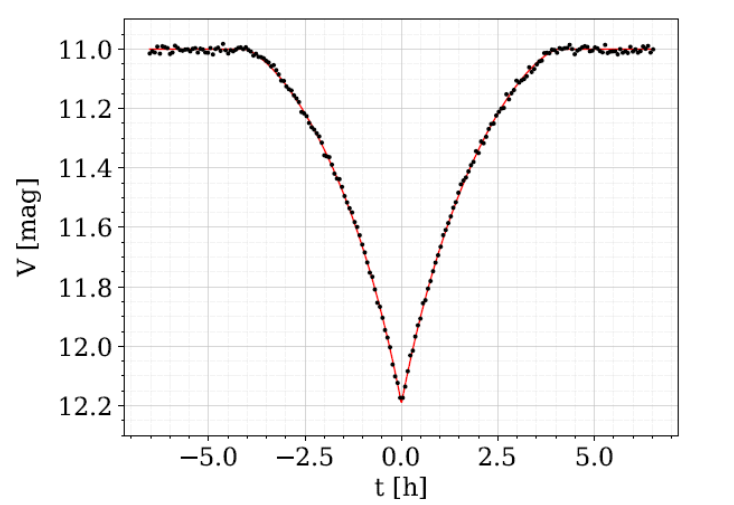
\includegraphics[height=8cm]{fig/1.png}
		\caption{Bolek系统的观测光变曲线. }
		\label{fig:1}
	\end{figure}
	
	\begin{figure}[!h]
		\centering
		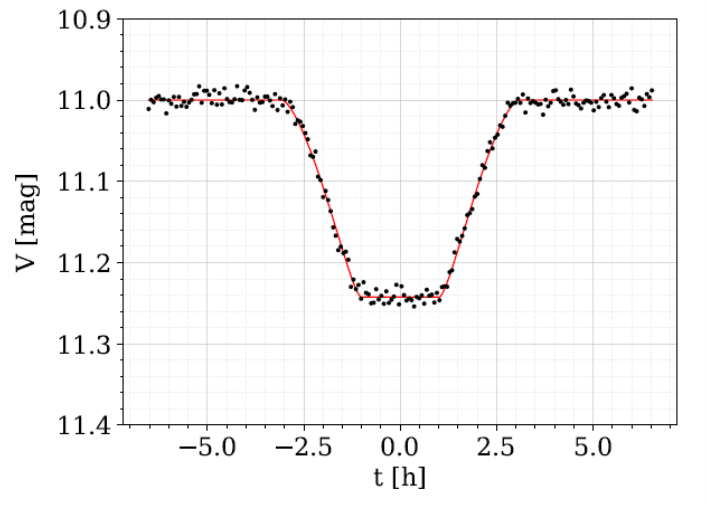
\includegraphics[height=8cm]{fig/2.png}
		\caption{Lolek系统的观测光变曲线. }
		\label{fig:2}
	\end{figure}
	
	在图中, \( t \) 是相对于最小红光时刻的时间 (小时), \( V \) 是在 \( V \)(可见光)波段的星等亮度. 点是测量值, 线是拟合的食的形状模型. 
	
	你可以假设在两种情况下食都是中心的(\( i = 90^\circ \)), 并且持续时间非常短暂, 边缘变暗可以忽略不计, 轨道偏心率很小. 
	
	在答题纸上, 画出每个次食的预测光变曲线形状. 写下你预测的方程式和计算过程. 
	
	\points{20}
	
	\section{毕宿五}
	
	1497年3月9日, Nicolaus Copernicus在博洛尼亚观测到了月亮遮掩毕宿五的天文现象. 
	在他的著作《天体运行论》(第六卷, 第27章)中, Copernicus描述了这一事件: ``我看见这颗星接触到月亮的暗边, 并在夜晚第五个小时结束时消失在月亮两角之间, 更靠近南角, 距离大约是月亮直径的三分之一. ''
	
	假设这次掩星是在当地时间子午线上观测到的, 那么在掩星最大时毕宿五位于月亮南边缘上方0.32角分, 并且从博洛尼亚看到的月亮视直径为31.5角分, 解决以下问题:
	
	\begin{enumerate}[label=(\alph*)]
		\item 找出与博洛尼亚处于同一经度的地方的纬度 $\varphi_1$, 从那里毕宿五会看起来从月亮中心后方经过. 
		
		\item 如果毕宿五看起来沿着月盘直径经过, 计算从纬度 $\varphi_1$ 观测到的掩星持续时间. 为了简化, 同样假设月亮和观测者以恒定速度做直线运动, 月亮的轨道是圆形的, 并且月亮的赤纬在掩星期间不变. \label{b}
		
		\item 对于位于纬度 $\varphi_1$ 的观测者, 在掩星期间找出月亮相对于背景恒星的地方视向速度, 以角分/小时为单位, 应用与部分 \ref{b} 相同的假设. 
		
		\item 估计在纬度 $\varphi_1$ 处, 月亮相对于背景恒星的地方视向速度的范围(以角分/小时为单位), 假设轨道是圆形的. 展示如何通过将月亮和观测者的相对速度表示为他们速度向量的函数来证明这一结果. 
	\end{enumerate}
	
	1497年毕宿五的赤纬是 $\delta_\mathrm{A} = 15.37^\circ$(由于岁差), 博洛尼亚的纬度是 $\varphi_\mathrm{B} = 44.44^\circ\text{ N}$. 
	
	\points{25}
	
	\section{星系团中的X射线发射}
	
	星系团是强大的X射线源. 已经确定发射机制是星系团内部高温氢和氦等离子体的热轫致辐射(自由-自由辐射). 等离子体的每个组分的光度 \( L_X \)(以W为单位)由以下公式描述:
	\[ L_X = 6 \times 10^{-41} N_e N_X T^{\frac{1}{2}} V Z_X^2, \]
	其中符号代表:
	\begin{description}
		\item[$X$ --] 氢(H)或氦(He),
		\item[$N_e$ --] 电子数密度 [\( \text{m}^{-3} \)], 
		\item[$N_X$ --] 离子X的数密度 [\( \text{m}^{-3} \)], 
		\item[$Z_X$ --] 离子X的原子序数, 
		\item[$T$ --] 等离子体的温度 [K], 
		\item[$V$ --] 等离子体所占体积 [\( \text{m}^3 \)]. 
	\end{description}
	
	\begin{enumerate}[label=(\alph*)]
		\item 假设等离子体完全电离, 每10个氢离子有1个氦离子;\( L_\mathrm{total} = 1.0 \times 10^{37} \text{ W} \);\( T = 80 \times 10^6 \text{ K} \);等离子体均匀分布在半径 \( R = 500 \text{ kpc} \) 的球体中;自吸收可以忽略不计. 确定发射X射线的等离子体的总质量(以太阳质量为单位). 
	\end{enumerate}
	\points{16}
	
	\vspace{-0em}
	宇宙微波背景(CMB)的光子与等离子体相互作用, 这个过程被称为逆Compton散射. CMB通常具有2.73 K温度下的热黑体辐射谱. 然而, 与等离子体的相互作用导致CMB谱的扭曲(被称为Sunyaev–Zeldovich效应). 
	
	\begin{enumerate}[label=(\alph*),start=2]
		\item 估算CMB光子在等离子体中的平均自由程, 即光子在与电子相互作用前平均行进的距离. 以Mpc为单位. 光子-电子相互作用的有效截面为 \(\sigma = 6.65 \times 10^{-29} \text{ m}^2\). \hfill(5分)
		
		\item 估算CMB光子的典型能量. \hfill(3分)
		
		\item 由于逆Compton散射, CMB光子的能量可以增加至多 \( (1+\beta)/(1-\beta) \) 的倍数, 其中 \( v = \beta c \) 是电子的速度. 估算散射CMB光子的能量. \hfill(6分)
	\end{enumerate}
	
	\points{共30}
	
	\section{DART}
	
	双小行星重定向测试(DART)是NASA的一个任务, 用于评估防御近地天体的行星防御方法. 航天器撞击了小行星Didymos的卫星Dimorphos, 以研究撞击如何影响其轨道. 
	
	\begin{enumerate}[label=(\alph*)]
		\item 假设碰撞是正面的、对心的, 并且完全非弹性的, 计算预期的轨道周期变化(以分钟为单位). 
		
		假设在撞击前Dimorphos以周期 \( P = 11.92 \text{ h} \) 绕Didymos在圆形轨道上运行. Dimorphos和Didymos的质量分别为 \(m = 4.3 \times 10^9 \text{ kg}\) 和 \( M = 5.6 \times 10^{11} \text{ kg} \). DART航天器在撞击瞬间相对于Dimorphos的质量和速度分别为 \(m_\mathrm{s} = 580 \text{ kg}\) 和 \( v_\mathrm{s} = 6.1 \text{ km s}^{-1} \). 忽略其他天体的引力影响. \points{20}
		
		\vspace{-1em}
		\item 事实上, Dimorphos的轨道周期观测到变化了 \( \Delta P_0 = -33 \text{ min} \). 这是由于与喷射出的碎片反冲相关的动量转移: 航天器被小行星吸收, 但撞击从小行星中挖掘出一些物质并将其喷射到太空中. 计算喷射出碎片的动量, 并将其表示为撞击前Dimorphos动量的一部分. 你可以假设喷射出物质的质量远小于Dimorphos的质量. \points{15}
		
		\vspace{-1em}
		\item 考虑到喷射出碎片的影响, 计算Dimorphos因撞击而导致的速度变化(以 \( \text{m ms}^{-1} \) 为单位). \points{5}
	\end{enumerate}
	\vspace{-1em}
	\points{共40}
	
	\section{LISA}
	
	激光干涉空间天线(LISA)是一个旨在探测低频引力波的提议实验. 它由三个以等边三角形排列的航天器组成. 通过引力波引起的航天器之间距离的变化可以被精确测量(详细说明见下文注释). 
	
	低频引力波的一个来源是致密双星系统, 例如双白矮星. 最近在距离太阳2.34 kpc的位置发现了这样一个系统. 该双星系统的轨道周期为414.79 s, 并且由于引力波的发射, 其周期变化率为 \(-7.49 \times 10^{-4} \text{ s yr}^{-1}\). 
	
	\begin{enumerate}[label=(\alph*)]
		\item 验证这个双星系统是否可以被LISA探测到. \hfill(25分)
		
		\item 计算啁啾质量. \hfill(5分)
		
		\item 确定两个子星的质量, 已知其中一个子星的半径与轨道半长轴的比率是0.139, 并假设两个子星都遵循下表给出的白矮星的质量-半径关系. \hfill(15分)
	\end{enumerate}
	\points{共45}
	
	\vspace{-1em}
	\textbf{注:}
	\begin{enumerate}
		\item 具有轨道周期 \( P \) 的双星系统以 \( f = 2/P \) 的频率发射引力波. 
		
		\item LISA测量一个无量纲量, 称为特征应变幅度 \( S \), 由下式给出:
		\[ S = h\sqrt{fT_\mathrm{obs}}, \]
		其中 \( T_\mathrm{obs} = 4\text{ yr} \) 是任务的预期持续时间. \( h \) 是引力波应变, 由下式给出:
		\[ h = \dfrac{2(G\mathcal{M})^{5/3}(\pi f)^{2/3}}{c^4D}, \]
		其中 \( \mathcal{M} \) 是所谓的啁啾质量, \( f \) 是引力波的频率, \( D \) 是到系统的距离. 如果我们用 \( M_1 \) 和 \( M_2 \) 表示双星的子星质量, 那么啁啾质量由下式给出:
		\[ \mathcal{M} = \dfrac{(M_1M_2)^{3/5}}{(M_1+M_2)^{1/5}}. \]
		下图展示了LISA对引力波频率的预期灵敏度. 
		
		\item 双星系统的半长轴 \( a \) 由于发射引力波而以以下速率变化:
		\[ \dfrac{\Delta a}{\Delta t} = -\dfrac{64}{5}\dfrac{G^3}{c^5}\dfrac{M_1M_2(M_1+M_2)}{a^3}. \]
	\end{enumerate}
	
	\begin{table}[!h]
		\centering
		\begin{tabular}{cc}
			\toprule
			$M$ ($M_\odot$) & $R$ ($R_\odot$)\\
			\midrule
			0.48&0.0144\\
			0.50&0.0147\\
			0.52&0.0150\\
			0.54&0.0153\\
			0.56&0.0156\\
			0.58&0.0159\\
			0.60&0.0162\\
			0.62&0.0165\\
			0.64&0.0168\\
			\bottomrule
		\end{tabular}
		\caption{根据Althaus 等人 (2013) 的理论模型, 此处列出的是$\log_g = 7.7$的白矮星的质量-半径关系. }
	\end{table}
	
	\begin{figure}[!h]
		\centering
		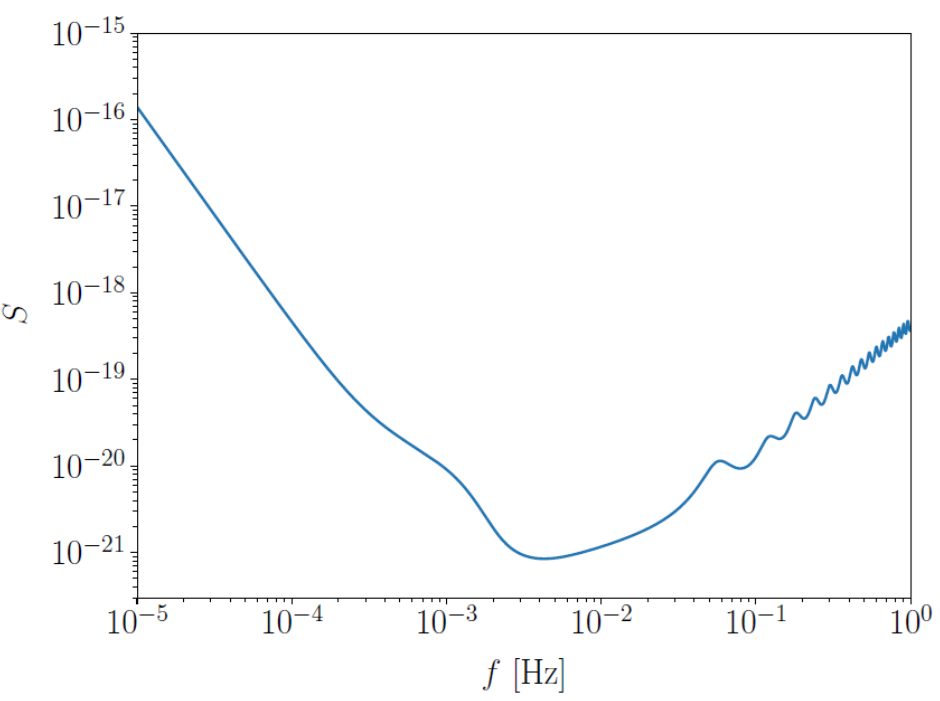
\includegraphics[height=8cm]{fig/3.png}
		\caption{LISA对引力波频率的预期灵敏度. }
	\end{figure}
	
\end{document}